\documentclass[12pt,letterpaper]{article}

\usepackage[utf8]{inputenc}
\usepackage[letterpaper,margin=1in]{geometry}
\usepackage{caption} % for table captions

\usepackage{amsmath} % for multi-line equations and piecewises
\usepackage{indentfirst} % to indent after a section
\usepackage{setspace}
\usepackage{times}
\usepackage{graphicx}
\usepackage{textcomp}
\usepackage{verbatim} % for block comments
\usepackage{subfig} % for subfigures
\usepackage{enumitem} % for a) b) c) lists
\usepackage{float}
\usepackage{titling}
\newcommand{\subtitle}[1]{%
  \posttitle{%
    \par\end{center}
    \begin{center}\large#1\end{center}
    \vskip0.5em}%
}
\usepackage{tikz}


\usetikzlibrary{shapes.geometric,arrows}
\tikzstyle{process} = [rectangle, rounded corners, minimum width=3cm, minimum height=1cm,text centered, draw=black, fill=blue!30]
\tikzstyle{arrow} = [thick,->,>=stealth]


\graphicspath{{images/}}
 
\usepackage[font={footnotesize,it}]{caption}
 



\setlength{\parindent}{15pt} % Default is 15pt.




\fontfamily{ptm}\selectfont

\title{Numerical Experiments for validating Non-Optimizing algorithms Report}
\subtitle{Draft 1}
\author{Jin Whan Bae and Gwendolyn Chee}
\date{2017-09-23}


\begin{document}
	
	\maketitle
	\hrule
	\onehalfspacing
	\thispagestyle{empty}

\section*{Introduction}
The main goal of the Demand-Driven Cycamore Archetype project is to develop in situ demand driven development schedule calculation through non-optimizing, deterministic-optimizing and stochastic-optimizing algorithms so Cyclus has the capability to deploy supporting fuel cycle facilities to enable a demand to be met.

These prediction models are being developed by University of South Carolina. In this report, we discuss how to design numerical experiments for testing the non-optimizing, deterministic and stochastic prediction methods. 

The first section evaluates the required tests for each kind of method assuming a once through fuel cycle. A once through nuclear fuel cycle refers to when spent fuel is not reprocessed. 

\section{Once through Nuclear Fuel Cycle}
\begin{figure}[H]
\caption{Flow Chart of Once through Nuclear Fuel Cycle}
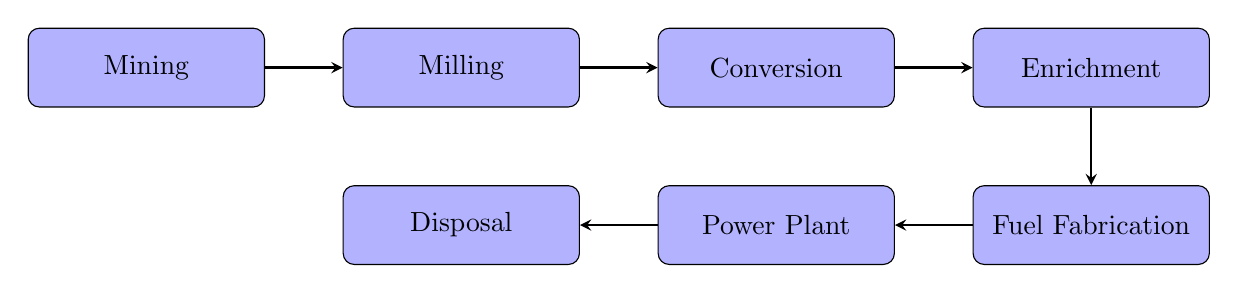
\begin{tikzpicture}[node distance=2cm]
\node (mining) [process] {Mining};
\node (milling) [process, right of=mining, xshift=2cm] {Milling};
\node (conversion) [process, right of=milling, xshift=2cm] {Conversion};
\node (enrichment) [process, right of=conversion, xshift=2cm] {Enrichment};
\node (fabrication) [process, below of=enrichment] {Fuel Fabrication};
\node (powerplant) [process, left of=fabrication, xshift = -2cm]{Power Plant};
\node (disposal) [process, left of=powerplant, xshift = -2cm]{Disposal};

\draw [arrow] (mining) -- (milling);
\draw [arrow] (milling) -- (conversion);
\draw [arrow] (conversion) -- (enrichment); 
\draw [arrow] (enrichment) -- (fabrication); 
\draw [arrow] (fabrication) -- (powerplant);
\draw [arrow] (powerplant) -- (disposal);
\end{tikzpicture}
\end{figure}

\subsection*{Non-optimizing method}
Conditions to Satisfy: 
\begin{itemize}
\item  Do all the reactors run? 
\item Is the input required by the reactors within a specific uncertainty of the analytic solution? 
\item  Is the output of the fuel fabrication facilities within a specific range of the input required by the reactors (calculated by the analytic solution) for all of them to run for each time step? 
\item  Is the output of the enrichment facilities within a specific range of the input required by the fuel fabrication facilities (calculated by the analytic solution) for each time step? 
\item Is the output of the conversion facilities within a specific range of the input required by the enrichment facilities (calculated by the analytic solution) for each time step? 
\item Is the output of uranium mining within a specific range of the input required by the conversion facilities (calculated by the analytic solution) for each time step? 
\item 
\end{itemize}

\subsection*{Deterministic-Optimizing method}

\end{document}






